% \documentclass[preview]{standalone}
\documentclass[tikz]{standalone}
\usepackage{amsmath,amssymb,amsthm,amsfonts}
\usepackage{tikz}
\usetikzlibrary{decorations.pathreplacing}
% \tikzexternalize
\begin{document}
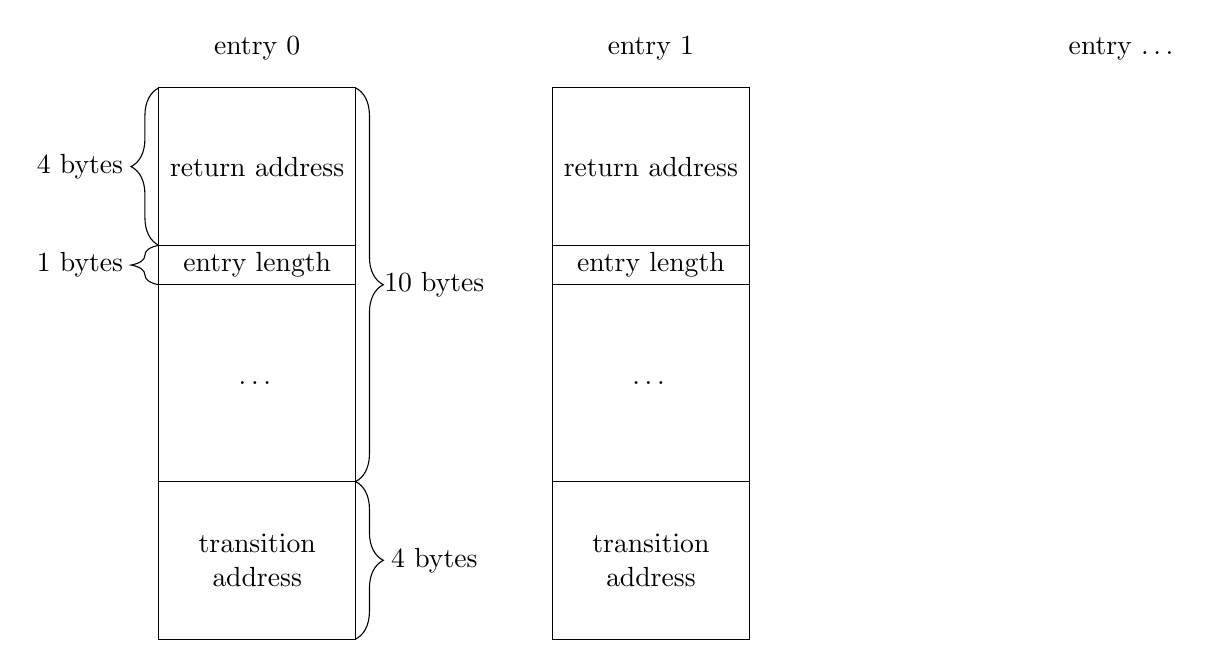
\begin{tikzpicture}
  % \draw[thick] (-1,0) rectangle +(6,7.5);
  % \draw (0,0) rectangle (4,2);
  % \draw (0,0) -- (10,10); % ...
  % \draw (10,0) -- (0,10); % ...
  % \node at (5,5) {Lorem ipsum at domine standalonus};
%   \node {root}
% child {node {left}}
% child {node {right}
% child {node {child}}
% child {node {child}}
% };
  \draw[align=center] (0,0) rectangle node{return address} (2.5,2);
  \draw[] (0,-0.5) rectangle node{entry length} (2.5,0);
  \draw[] (0,-3) rectangle node{$\dots$} (2.5,-0.5);
  \draw[align=center] (0,-5) rectangle node{transition \\ address} (2.5,-3);
  \draw[decorate,decoration={brace,amplitude=10pt}] (0,0) -- (0,2) node[black,midway,xshift=-1cm] {$4$ bytes};
  \draw[decorate,decoration={brace,amplitude=10pt}] (0,-0.5) -- (0,0) node[black,midway,xshift=-1cm] {$1$ bytes};
  \draw[decorate,decoration={brace,amplitude=10pt,mirror}] (2.5,-3) -- (2.5,2) node[black,midway,xshift=1cm] {$10$ bytes};
  \draw[decorate,decoration={brace,amplitude=10pt,mirror}] (2.5,-5) -- (2.5,-3) node[black,midway,xshift=1cm] {$4$ bytes};
  \draw[] (1.25,2.5) node{entry $0$};

  \draw[align=center] (5,0) rectangle node{return address} (7.5,2);
  \draw[] (5,-0.5) rectangle node{entry length} (7.5,0);
  \draw[] (5,-3) rectangle node{$\dots$} (7.5,-0.5);
  \draw[align=center] (5,-5) rectangle node{transition \\ address} (7.5,-3);
  % \draw[decorate,decoration={brace,amplitude=10pt}] (5,0) -- (5,4) node[black,midway,xshift=-1cm] {$4$ bytes};
  % \draw[decorate,decoration={brace,amplitude=10pt}] (5,-1) -- (5,0) node[black,midway,xshift=-1cm] {$1$ bytes};
  % \draw[decorate,decoration={brace,amplitude=10pt,mirror}] (7.5,-6) -- (7.5,4) node[black,midway,xshift=1cm] {$10$ bytes};
  % \draw[decorate,decoration={brace,amplitude=10pt,mirror}] (7.5,-10) -- (7.5,-6) node[black,midway,xshift=1cm] {$4$ bytes};
  \draw[] (6.25,2.5) node{entry $1$};

  % \draw[align=center] (10,0) rectangle node{return address} (12.5,4);
  \draw[] (12.25,2.5) node{entry $\dots$};
  % \draw[] (12.25,-3.5) node{$\dots$};
\end{tikzpicture}

\end{document}